\documentclass[12pt, notitlepage, final]{article} 

\newcommand{\name}{Vince Coghlan}

\usepackage{amsfonts}
\usepackage{amssymb}
\usepackage{amsmath}
\usepackage{latexsym}
\usepackage{enumerate}
\usepackage{amsthm}
\usepackage{nccmath}
\usepackage{setspace}
\usepackage[pdftex]{graphicx}
\usepackage{epstopdf}
\usepackage[siunitx]{circuitikz}
\usepackage{tikz}
\usepackage{float}
\usepackage{cancel} 
\usepackage{setspace}
\usepackage{overpic}
\usepackage{mathtools}
\usepackage{listings}
\usepackage{color}

\numberwithin{equation}{section}
\DeclareRobustCommand{\beginProtected}[1]{\begin{#1}}
\DeclareRobustCommand{\endProtected}[1]{\end{#1}}
\newcommand{\dbr}[1]{d_{\mbox{#1BR}}}
\newtheorem{lemma}{Lemma}
\newtheorem*{corollary}{Corollary}
\newtheorem{theorem}{Theorem}
\newtheorem{proposition}{Proposition}
\theoremstyle{definition}
\newtheorem{define}{Definition}
\newcommand{\column}[2]{
\left( \begin{array}{ccc}
#1 \\
#2
\end{array} \right)}

\newdimen\digitwidth
\settowidth\digitwidth{0}
\def~{\hspace{\digitwidth}}

\setlength{\parskip}{1pc}
\setlength{\parindent}{0pt}
\setlength{\topmargin}{-3pc}
\setlength{\textheight}{9.0in}
\setlength{\oddsidemargin}{0pc}
\setlength{\evensidemargin}{0pc}
\setlength{\textwidth}{6.5in}
\newcommand{\answer}[1]{\newpage\noindent\framebox{\vbox{{\bf ECEN 3400 Spring 2014} 
\hfill {\bf \name} \vspace{-1cm}
\begin{center}{Project}\end{center} } }\bigskip }

%absolute value code
\DeclarePairedDelimiter\abs{\lvert}{\rvert}%
\DeclarePairedDelimiter\norm{\lVert}{\rVert}
\makeatletter
\let\oldabs\abs
\def\abs{\@ifstar{\oldabs}{\oldabs*}}
%
\let\oldnorm\norm
\def\norm{\@ifstar{\oldnorm}{\oldnorm*}}
\makeatother

\def\dbar{{\mathchar'26\mkern-12mu d}}
\def \Frac{\displaystyle\frac}
\def \Sum{\displaystyle\sum}
\def \Int{\displaystyle\int}
\def \Prod{\displaystyle\prod}
\def \P[x]{\Frac{\partial}{\partial x}}
\def \D[x]{\Frac{d}{dx}}
\newcommand{\PD}[2]{\frac{\partial#1}{\partial#2}}
\newcommand{\PF}[1]{\frac{\partial}{\partial#1}}
\newcommand{\DD}[2]{\frac{d#1}{d#2}}
\newcommand{\DF}[1]{\frac{d}{d#1}}
\newcommand{\fix}[2]{\left(#1\right)_#2}
\newcommand{\ket}[1]{|#1\rangle}
\newcommand{\bra}[1]{\langle#1|}
\newcommand{\braket}[2]{\langle #1 | #2 \rangle}
\newcommand{\bopk}[3]{\langle #1 | #2 | #3 \rangle}
\newcommand{\Choose}[2]{\displaystyle {#1 \choose #2}}
\newcommand{\proj}[1]{\ket{#1}\bra{#1}}
\def\del{\vec{\nabla}}
\newcommand{\avg}[1]{\langle#1\rangle}
\newcommand{\piecewise}[4]{\left\{\beginProtected{array}{rl}#1&:#2\\#3&:#4\endProtected{array}\right.}
\newcommand{\systeme}[2]{\left\{\beginProtected{array}{rl}#1\\#2\endProtected{array}\right.}
\def \KE{K\!E}
\def\Godel{G$\ddot{\mbox{o}}$del}

\onehalfspacing

\begin{document}
\answer{}

A typical rebar (metric gauge \#36) has a mass of 8kg/m and you can assume that each bar is 10m
long and that 10 bars are tied and lifted at the same time. The nominal diameter of a \#36 rebar is
36mm.


\textbf{1. Magnetic Field Intensity (H):} What magnetic field intensity ($H$) along
the axis of the crane's lifter thingy will be generated by a
crane with a magnetic coil of radius $1m$, $2000$ coils, with a current of $100mA$ flowing through it?  Assume
that the bundle of rebar is $2m$ away.

\textbf{Solution:}  We can apply the Biot-Savart law on one loop to find the outward component of the field.
Note that all other fields will cancel due to the symmetry of the coil:
\[
  dH_z=\frac{IdL}{4\pi}\frac{R}{(r^2+R^2)^{3/2}}
\]
Where $I$ is current, $dL$ is a point on the loop, $R$ is the radius of the coil, $r$ is the distance from the
coil, and $\pi$ is $\pi$.  Integrating over the loop we find that:
\[
  H_z=\frac{2\pi R^2 I}{4\pi(r^2+R^2)^{3/2}} = \frac{R^2I}{2(r^2+R^2)^{3/2}}
\]
We can then multiply by $N$ turns to find:
\[
  H_z=\frac{NR^2I}{2(r^2+R^2)^{3/2}}
\]
Substituting values we find that:
\[
  H_z=\frac{2000\cdot(1)^2\cdot0.1}{2(2^2+(1)^2)^{3/2}} = 8.944 A/m
\]

\textbf{2. Ampere's Law:} Assume that the magnetic coil is a two meter long solenoid, what is the magnetic
flux density ($B$) at a distance of $0.7m$ from the bottom end? how about $1.5m$?  Assume that the other values are
the same as in problem 1.

\textbf{Solution:}  Use amperes law to find the magnetic field inside a solenoid.  This means defining an
integration path like so:
\begin{figure}[H]
\begin{center}
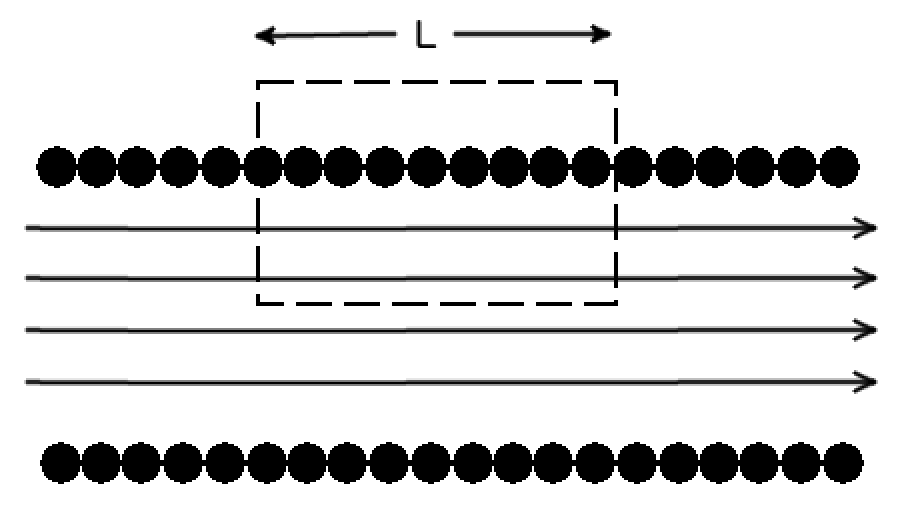
\includegraphics[width=8cm]{f1}
\end{center}
\end{figure}
And applying Amperes law to this path, first, find the integral:
\[
  \int_AB\cdot dL = BL
\]
Where $L$ is the horizontal length of the integration path.  The current inclosed is $N\cdot I$ Where $N$ is the
number of turns in the area of integration $A$.  Ampere's law tells us that these things are equal, and:
\[
  BL=\mu_0NI \Rightarrow B=\mu_0\frac{N}{L}I
\]
Note that $\frac{N}{L}$ is just the amount of loops per unit length.  Substituting in our values we find:
\[
  B = (4\pi\cdot10^{-7})(\frac{2000}{2})(0.1) = 125.66 \mu T
\]
Regardless of where we are in the solenoid, proving that the field is uniform inside the solenoid.

\textbf{3. Magnetic Flux Density (B):} Assuming all previous values (except that the magnetic coil is not
two meters long, but a very small width), what is the magnetic flux density $B$ a
distance of 5m away along the axis of the crane lifter thingy?

\textbf{Solution:} We know that $B=\mu H$, Thus we can use our solution from problem 1:
\[
  B = \mu H = \frac{\mu NR^2I}{2(r^2+R^2)^{3/2}} = \frac{(4\pi\cdot10^{-7})2000\cdot(1)^2\cdot0.1}{2(5^2+(1)^2)^{3/2}} = 0.948\mu T
\]

\newpage

\textbf{4. Magnetic Flux:} What is the magnetic flux through the crane's coil?

\textbf{Solution:} Since the field is uniform, the flux is just the flux density devided by the area:
\[
  \Phi = B\cdot A = \frac{N\mu I (\pi R^2)}{2R} = \frac{2000\cdot0.1\cdot4\pi\cdot10^{-7}\cdot\pi}{2} = 394.8\mu T
\]

\textbf{5. B(H) Dependence in Linear and Nonlinear Materials:} Assume for this problem that the coil inside
the crane is a wire wrapped around a thin toroidal core made out of a nonlinear material where the the initial
magnetization curve can be approximated by the function $B(H) = B_0H/(H_0+H)$ where the coefficients are $B_0=1.37T$
and $H_0=64A/m$.  Find B(H) as a function of current given that the core has been wrapped 2000 times and has a
radius of 1 meter.

\textbf{Solution:} We can first find $H$ in the core with amperes law to be:
\[
  H = \frac{NI}{2\pi R}
\]
With this we can substitute in to find:
\[
  B(H) = \frac{B_0N\cdot I}{2\pi R H_0 + N\cdot I}
\]
With the numbers:
\[
  B(H) = \frac{1.37I}{I+0.20106}
\]

\textbf{6. Inductance:} The local strongman decides to stop by the job site to bend rebar.  He bends a piece of rebar
into a perfect circle around the torroidal coil of the crane, perpendicular to the coil.  He then holds it there to
show off to the nearby constuction workers.  Assume the torroidal coil is 0.1m tall and 0.1m wide with a inner
radius of 1 meter.  After the strongman preforms his feat, the worker in the crane decides to mess with him, and turns
the coil on from a current of 0A to a current of 1A in a duration of 1 second.  What is the current in the rebar during
this one second?  Assume that the rebar has a resistance of $100\Omega$ and that there are 2000 wraps of wire around the
core.

\textbf{Solution:} The radius of the now bent rebar is $R=\frac{1}{2\pi}=0.159m$. We can obtain the flux:
\[
  \Phi = \int_a^b \frac{\mu_0NI(t)h}{2\pi}\frac{dr}{r} = \frac{\mu_0NI(t)h}{2\pi}\ln\frac{b}{a}
\]
We can then find the induced voltage:
\[
  e=-\frac{d}{dt}\frac{\mu_0NI(t)h}{2\pi}\ln\frac{b}{a} = -\frac{\mu_0Nh}{2\pi}\ln\frac{b}{a}
\]
The current is thus:
\[
  I=\frac{V}{R}=-\frac{\mu_0Nh}{2\pi R}\ln\frac{b}{a}=-\frac{\mu_0(2000)(0.1)}{2\pi 100}\ln\frac{1.1}{1} = -3.812 \cdot10^{-8} A
\]

\textbf{7. Magnetic Energy:} What is the energy required to start up the coil from problem 5?

\textbf{Solution:} We know:
\[
  \text{Energy Stored} = \frac{1}{2} L I^2
\]
We found inductance in problem 5 to be:
\[
  L = \frac{\mu N h}{2\pi}\ln\frac{b}{a}
\]
So we know that the energy in the coil is:
\[
  E = \frac{\mu N h I^2}{4\pi}\ln\frac{b}{a} = 1.91\cdot10^{-6} J
\]
\enlargethispage{\baselineskip}
\textbf{8. Magnetic Forces:} The strongman decides to preform more feats of strength and will.  The crane picks up
the bent peice of rebar, how much force is requred by the strongman's toned muscles to remove this?  Recall that the
radius of the coil is $1m$, the coil is now a very thin solenoid of 2000 wraps, the current flowing through the coil
is $1 A$, the weight of the rebar is 10 kg.


\textbf{Solution:} We first find the force using the equation in the textbook:
\[
  F=\frac{1}{2}\frac{B^2}{\mu_0}2S = \frac{\Phi}{\mu_0 S}
\]
Where S is the area of the coil. We know from problem 4 that:
\[
  \Phi=\frac{N\mu I(\pi R^2)}{2R}
\]
S is $\pi R^2$.  This means that the force required is:
\[
  F_{sm} = F_{mag} - F_{bar} = \frac{N\mu I(\pi R^2)}{2R(\mu \pi R^2)} - 10(9.8) = 902 N
\]


\textbf{Part 2: Ground Fault Interrupt and GFCI.}

Ground fault interrupters are used mostly to protect people and devices from electrical shock.  When there is a difference
in the currents of the two differenct wires from a power source, it indicates that a short has occured, and it immidiately
trips the circuit so that no more current is delivered.  It can detect a few milliamperes difference.  It does this using
some really cool E \& M.  The hot and neutral wires of a AC power source are passed through a solenoid.  Since the current
in the two wires is going in opposite directions, there is a net zero current, which, due to Ampere's law, means a net
zero induced current.  If there is a difference in these two currents, then the current in the solenoid will go in one
direction of the other, meaning a short has occured.  This is then detected, and both currents are cut.  In order to
cut the current, it uses another solenoid.  When the current in the detecting coil has reached the specific value, a
comparator circuit sends a large amount of current to another solenoid attached to a small piston.  This whole detection
and reaction can occur in as little as one-thirtieth of a second.  All of this information was obtained from
http://home.howstuffworks.com/question117.htm and http://hyperphysics.phy-astr.gsu.edu/hbase/electric/gfi2.html. A
diagram I made can be seen below.

\begin{figure}[H]
\begin{center}
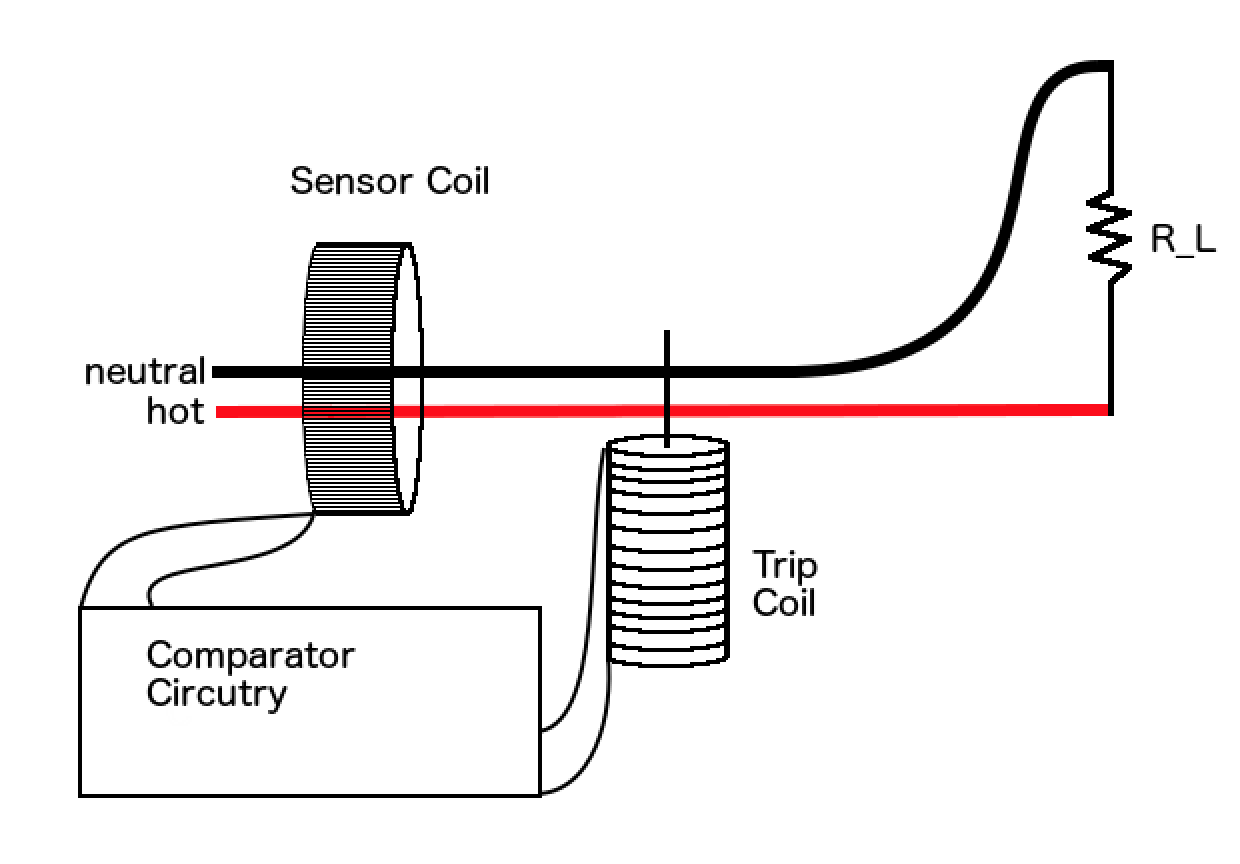
\includegraphics[width=14cm]{f2}
\end{center}
\end{figure}


\end{document}
